\documentclass[11pt]{article}

\usepackage[margin=1in]{geometry}
\usepackage{amsmath}
\usepackage{amssymb}
\usepackage{array}
\usepackage{booktabs}
\usepackage{graphicx}
\usepackage{longtable}
\usepackage{url}
\usepackage[hidelinks]{hyperref}

\newcommand{\methodname}{Fixed Heavy-Tailed Forecasting}
\newcommand{\studenthead}{fixed Student-$t$ head}
\newcommand{\gaussianhead}{Gaussian head}
\newcommand{\nll}{NLL}
\newcommand{\crps}{CRPS}
\newcommand{\mse}{MSE}
\newcommand{\mae}{MAE}
\newcommand{\rmse}{RMSE}
\newcommand{\etal}{et al.\ }
\newcommand{\best}[1]{\textbf{#1}}
\newcommand{\dataset}[1]{\textsc{#1}}

\newcommand{\papertitle}{Fixed Heavy-Tailed Probabilistic Forecasting under Missing Historical Observations}
\newcommand{\paperauthors}{Anonymous Authors}


\setlength{\parindent}{1.2em}
\setlength{\parskip}{0.25em}
\setlength{\emergencystretch}{3em}

\begin{document}

\title{\papertitle}
\author{\paperauthors}
\date{}
\maketitle

\begin{abstract}
Probabilistic forecasting from missing historical observations requires both accurate predictions and uncertainty estimates that remain meaningful under controlled input corruption. We introduce a leakage-controlled fixed missing-history evaluation protocol with train-only normalization, fixed validation and test masks, and no masking of future targets. Within this protocol, we study a lightweight fixed Student-$t$ head with degrees of freedom fixed at 8. It has the same trainable parameter count as matched Gaussian and Laplace heads. On TimePerceiver, Student-$t$ variants improve negative log-likelihood (NLL) and continuous ranked probability score (CRPS) across three datasets and four probability-head training seeds, with all 12 paired comparisons meeting the predefined point-noninferiority criterion. A distribution-head ablation shows that fixed df=8 is sufficient under the evaluated setting, while learned per-channel degrees of freedom add no consistent benefit. On PatchTST, the fixed Student-$t$ head improves NLL and CRPS on all three datasets. However, Electricity mean squared error (MSE) increases by 1.194\%, slightly exceeding the pre-registered 1\% tolerance, so the complete second-backbone gate is not positive. We also retain two negative findings: global-statistics feature-wise linear modulation does not outperform a capacity-matched static adapter, and additive split conformal calibration does not improve native intervals in the tested condition. The evidence is limited to two backbones, three datasets, fixed masks, and restricted seed coverage; it supports probabilistic-score robustness rather than complete metric-wise invariance.

\end{abstract}

\section{Introduction}
\label{sec:introduction}

Forecasting systems often receive incomplete histories. Sensors fail, communication channels drop observations, and data pipelines can produce blocks or channels of missing values. A useful forecasting model must therefore operate on a partially observed historical window and quantify uncertainty about an unobserved future. These requirements are distinct: a point forecast can remain plausible while its predictive distribution becomes too narrow, too light-tailed, or otherwise poorly matched to the residuals.

Many missing-data studies focus on reconstructing the history before evaluating a downstream task. Imputation is important, but reconstruction quality alone does not determine forecast quality. A forecasting-centered evaluation must hold the historical mask fixed across methods, keep future targets outside the input, and prevent test statistics from entering normalization or model selection. Without these controls, apparent differences can reflect mask resampling or leakage rather than the predictive method.

Gaussian likelihoods are attractive because they are simple and differentiable. Their tails can nevertheless assign excessive negative log-likelihood to large standardized residuals. A Student-$t$ likelihood offers heavier tails while retaining a familiar location-scale parameterization. Fixing its degrees of freedom removes the need to estimate an additional shape parameter and makes capacity matching straightforward. Proper scoring rules, including log score and the continuous ranked probability score, provide complementary views of probabilistic quality \cite{gneiting2007proper}.

This study combines a fixed missing-history protocol with a lightweight fixed Student-$t$ head. The historical observation mask is treated as an evaluation asset rather than an ephemeral random draw. Gaussian, Laplace, and fixed Student-$t$ heads use matched trainable location-scale projections. We retain negative results for a missingness-aware feature-wise linear modulation (FiLM) adapter and an additive split-conformal procedure. The goal is an auditable account of what improves, what does not, and where a tradeoff remains.

The main evidence uses TimePerceiver \cite{lee2025timeperceiver} on ETTh1, Weather, and Electricity. Across four probability-head training seeds, Student-$t$ variants improve NLL and CRPS in all 12 paired cells and meet point noninferiority in all 12. A controlled ablation supports fixed df=8 as sufficient. A second study uses PatchTST \cite{nie2023patchtst}. Its fixed Student-$t$ head improves NLL and CRPS on all three datasets, but Electricity MSE rises from 0.165829 to 0.167809. The 1.194\% increase exceeds the pre-registered 1\% tolerance, so the full multi-metric gate remains negative.

The contributions are threefold:
\begin{enumerate}
    \item We define a leakage-controlled fixed missing-history evaluation protocol for deterministic and probabilistic forecasting.
    \item We study a lightweight fixed Student-$t$ probability head with the same trainable parameter count as matched Gaussian and Laplace heads.
    \item We provide a cross-backbone empirical study with a distribution ablation, retained negative results, and an explicit PatchTST Electricity point-prediction tradeoff.
\end{enumerate}

\section{Related Work}
\label{sec:related}

\subsection{Probabilistic time-series forecasting}

Neural probabilistic forecasters learn predictive distributions rather than only conditional means. DeepAR, for example, trains a shared autoregressive recurrent model over related series and optimizes a parametric likelihood \cite{salinas2020deepar}. Such models make distributional assumptions explicit and enable evaluation with proper scoring rules. Log score assesses predictive density at the realized target, while CRPS evaluates the full univariate cumulative distribution \cite{gneiting2007proper}. Our study adopts both scores and also reports point metrics from the predictive location.

\subsection{Heavy-tailed predictive distributions}

Location-scale likelihoods differ primarily in how they allocate mass away from the center. A Gaussian density decays rapidly, a Laplace density has exponential tails, and a Student-$t$ density has polynomial tails. The degrees of freedom control the Student-$t$ tail weight. We compare these families under matched location-scale capacity. Unlike an adaptive shape model, our selected form fixes df=8 and introduces no trainable degrees-of-freedom parameter.

\subsection{Forecasting with missing historical observations}

Time-series missingness has often been addressed through imputation. BRITS learns missing values in a bidirectional recurrent system and evaluates downstream prediction tasks \cite{cao2018brits}. CSDI instead models a conditional distribution over missing values with score-based diffusion and supports probabilistic imputation \cite{tashiro2021csdi}. These methods motivate careful treatment of observation masks. Our protocol asks a narrower question: given a fixed incomplete history, how do point and probabilistic forecast metrics change when the forecasting head changes? We do not present a new imputation method.

\subsection{Conformal prediction for time series}

Conformal methods transform calibration residuals into prediction sets under explicit assumptions about calibration and test examples. Time-series extensions address multi-horizon forecasting and weakened exchangeability conditions \cite{stankeviciute2021conformal}. Our conformal experiment is deliberately limited to an additive split procedure with a strict temporal split and embargo. Its negative outcome is specific to that design and does not generalize to other conformal scores or online methods.

\subsection{General-purpose forecasting backbones}

TimePerceiver uses latent bottlenecks and timestamp-aligned decoder queries to support multiple temporal prediction layouts \cite{lee2025timeperceiver}. PatchTST tokenizes temporal patches and shares Transformer weights across channels \cite{nie2023patchtst}. They provide structurally different frozen backbones for the present head comparison. We treat their clean checkpoints as fixed feature extractors and avoid ranking the two architectures by their absolute metrics.

\section{Problem Formulation}
\label{sec:problem}

Let $X \in \mathbb{R}^{L \times C}$ denote a historical multivariate sequence with input length $L$ and $C$ channels. Let $Y \in \mathbb{R}^{H \times C}$ denote the future target over forecast horizon $H$. A binary historical observation mask $M \in \{0,1\}^{L \times C}$ indicates which elements of $X$ are observed. The masked historical input is
\begin{equation}
    \widetilde{X} = M \odot X + (1-M) \odot v_{\mathrm{miss}},
    \label{eq:masked-input}
\end{equation}
where $v_{\mathrm{miss}}$ is the protocol's missing-value representation and $\odot$ denotes elementwise multiplication.

The mask acts only on historical inputs. The future target $Y$ is never masked, copied into $\widetilde{X}$, or used to construct the input mask. Normalization parameters are fitted on the training split only and then reused for validation and test data. Validation and test masks are fixed assets, so matched methods receive identical observed histories.

A backbone maps $\widetilde{X}$, time features, and the observation mask to forecast features $Z$. A probability head then defines a marginal predictive density for each target element:
\begin{equation}
    p(Y \mid \widetilde{X}, M)
    = \prod_{h=1}^{H}\prod_{c=1}^{C}
      p\!\left(Y_{h,c}\mid Z_{h,c}\right).
    \label{eq:marginal-factorization}
\end{equation}
Equation~\ref{eq:marginal-factorization} is a modeling factorization for marginal target distributions. It does not represent cross-channel or cross-horizon covariance, and its marginal intervals do not imply simultaneous coverage.

We evaluate point accuracy with mean squared error (MSE), mean absolute error (MAE), and root mean squared error (RMSE). We evaluate predictive distributions with negative log-likelihood (NLL), CRPS, interval coverage, interval width, and interval score. Lower values are better for all listed metrics except coverage, which is compared with its nominal target.

For a candidate head $a$ and a matched Gaussian reference $g$, point noninferiority requires
\begin{equation}
    \frac{\mathrm{MSE}_{a}-\mathrm{MSE}_{g}}{\mathrm{MSE}_{g}}
    \leq 0.01.
    \label{eq:point-gate}
\end{equation}
The 1\% threshold is pre-registered for the paired comparisons and is not changed after observing test results.

\section{Method}
\label{sec:method}

\subsection{Backbone and probability-head interface}

The method operates on forecast features produced by a frozen backbone. For TimePerceiver, these features follow the model's latent encoder and query-based decoder \cite{lee2025timeperceiver}. For PatchTST, they follow the supervised patch encoder \cite{nie2023patchtst}. We do not alter either backbone architecture. A small output head maps each feature vector to the parameters of a marginal predictive distribution.

\subsection{Gaussian reference}

The Gaussian reference predicts a location $\mu$ and an unconstrained scale value $s$. Its positive scale is
\begin{equation}
    \sigma = \operatorname{softplus}(s) + 10^{-4}.
    \label{eq:scale}
\end{equation}
The head is trained by minimizing mean Gaussian NLL over observed target elements. Because future targets are complete in this protocol, the target mask does not remove forecast elements.

\subsection{\texorpdfstring{Fixed Student-$t$ head}{Fixed Student-t head}}

The fixed Student-$t$ head predicts the same location $\mu$ and scale $\sigma$ as the Gaussian reference. It sets the degrees of freedom to
\begin{equation}
    \nu = 8
    \label{eq:fixed-df}
\end{equation}
for every target channel and horizon. There is no trainable degrees-of-freedom parameter. The NLL objective follows the univariate Student-$t$ density independently for each target element.

The fixed value is a reference setting shown to be empirically sufficient by the distribution-head ablation before the PatchTST experiment. It was retained for Gate 5b without dataset-specific retuning. We do not describe df=8 as theoretically optimal.

\subsection{Capacity matching}

Gaussian, Laplace, and fixed Student-$t$ heads use identical trainable location and scale projections. They therefore have the same trainable parameter count for a given backbone and dataset. Their difference lies in the likelihood and interval quantiles, not in the number of optimized weights. A learned-df Student-$t$ variant adds one degrees-of-freedom parameter per target channel and is used only in the controlled ablation and TimePerceiver multi-seed evidence.

\subsection{Evaluation protocol}

Every paired head comparison uses the same backbone checkpoint, train/validation/test split, normalization statistics, validation mask, test mask, optimization budget, and checkpoint-selection rule. The test set is evaluated only after selecting the lowest validation-NLL checkpoint. NLL and CRPS provide the primary probabilistic comparison, while Equation~\ref{eq:point-gate} guards against a material point-prediction regression.

\section{Experimental Setup}
\label{sec:setup}

\subsection{Datasets and deterministic references}

We evaluate ETTh1, Weather, and Electricity. Every experiment uses input length 384 and prediction length 96. We retain the official train, validation, and test boundaries for each dataset. Normalization statistics are fitted on the training split only and then frozen. Table~\ref{tab:clean-baselines} records the clean-input TimePerceiver references used to quantify degradation under missing history.

\begin{table}[t]
    \centering
    \caption{Clean-input TimePerceiver references. Metrics are reproduced under the project protocol with one official training seed per dataset.}
    \label{tab:clean-baselines}
    \small
    \begin{tabular}{@{}lrrrr@{}}
\toprule
Dataset & MSE & MAE & RMSE & Best epoch \\
\midrule
ETTh1 & 0.374462 & 0.398943 & 0.611933 & 26 \\
Weather & 0.144059 & 0.199637 & 0.379550 & 38 \\
Electricity & 0.125364 & 0.220123 & 0.354068 & 60 \\
\bottomrule
\end{tabular}

\end{table}

\subsection{Missing-history protocol}

Historical masking uses random, block, channel, and mixed masks at missing rates 0.1, 0.3, 0.5, and 0.7. Validation and test masks are generated once and reused across matched models. The fixed test-mask seed is 2025. Training masks follow the recorded deterministic seed rule for each formal experiment. Missingness changes only the historical input. Future targets remain complete and are never available to the model.

\subsection{Probability-head training}

TimePerceiver comparisons keep the official backbone checkpoint fixed and vary the probability-head training seed over 2021, 2022, 2023, and 2025. This is a four-seed head study rather than full end-to-end backbone retraining. The broader cross-condition and distribution-ablation experiments use seed 2025 unless stated otherwise.

PatchTST uses one clean-backbone training seed and one probability-head seed, both 2025. Its second-backbone comparison is limited to random missingness at rate 0.3. Gaussian and fixed Student-$t$ heads share the backbone checkpoint, split, masks, optimizer budget, and validation-based checkpoint rule.

\subsection{Metrics and model selection}

We report NLL, CRPS, MSE, MAE, RMSE, prediction-interval coverage probability (PICP), mean prediction-interval width (MPIW), and interval score. CRPS uses 64 Monte Carlo (MC) samples with MC seed 52025. Native intervals come directly from each predictive distribution. Early stopping and checkpoint selection use validation NLL. Test metrics are not used for training, hyperparameter selection, or early stopping.

For paired gates, lower NLL is a probabilistic win. CRPS must be noninferior under the registered comparison rule, and relative MSE degradation must not exceed 1\%. We report each component separately rather than collapsing a partial pass into a positive overall decision.

\section{Results}
\label{sec:results}

\subsection{Deterministic degradation under missing history}
\label{sec:degradation}

The fixed-mask deterministic audit contains 48 dataset, mask-type, and missing-rate cells. Across the 12 dataset-by-mask-type curves, MSE increases monotonically over the evaluated missing rates. Table~\ref{tab:fixed-mask-degradation} gives the representative matrix retained in the main text, and Figure~\ref{fig:missingness-degradation} visualizes the degradation. The complete matrix appears in Appendix~\ref{app:additional-results}.

\begin{table}[t]
    \centering
    \caption{Forecast degradation under fixed historical masks. Relative degradation is measured against the corresponding clean TimePerceiver reference.}
    \label{tab:fixed-mask-degradation}
    \scriptsize
    \begin{tabular}{@{}lrrrr@{}}
\toprule
Dataset & Mask & Rate & MSE & Clean degradation \\
\midrule
ETTh1 & Block & 0.30 & 0.423837 & 13.19\% \\
ETTh1 & Channel & 0.30 & 0.583704 & 55.88\% \\
ETTh1 & Mixed & 0.30 & 0.495055 & 32.20\% \\
ETTh1 & Random & 0.10 & 0.378811 & 1.16\% \\
ETTh1 & Random & 0.30 & 0.425394 & 13.60\% \\
ETTh1 & Random & 0.50 & 0.525856 & 40.43\% \\
Electricity & Block & 0.30 & 0.184630 & 47.28\% \\
Electricity & Channel & 0.30 & 0.391038 & 211.92\% \\
Electricity & Mixed & 0.30 & 0.246785 & 96.86\% \\
Electricity & Random & 0.10 & 0.138429 & 10.42\% \\
Electricity & Random & 0.30 & 0.200572 & 59.99\% \\
Electricity & Random & 0.50 & 0.325732 & 159.83\% \\
Weather & Block & 0.30 & 0.180420 & 25.24\% \\
Weather & Channel & 0.30 & 0.284471 & 97.47\% \\
Weather & Mixed & 0.30 & 0.224939 & 56.14\% \\
Weather & Random & 0.10 & 0.169631 & 17.75\% \\
Weather & Random & 0.30 & 0.240810 & 67.16\% \\
Weather & Random & 0.50 & 0.331313 & 129.99\% \\
\bottomrule
\end{tabular}

\end{table}

\begin{figure}[t]
    \centering
    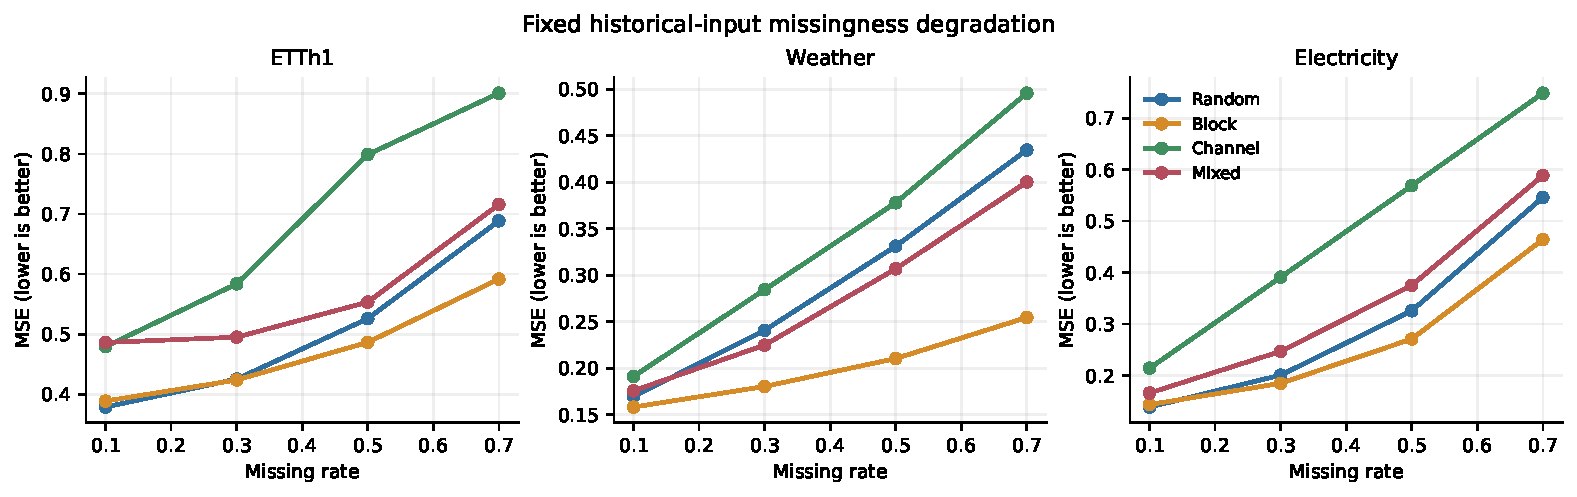
\includegraphics[width=0.96\linewidth]{figures/fig1_missingness_degradation.pdf}
    \caption{MSE under the fixed missing-history evaluation. Higher missing rates increase error across the evaluated datasets and mask types.}
    \label{fig:missingness-degradation}
\end{figure}

\subsection{TimePerceiver probabilistic forecasting}
\label{sec:timeperceiver-results}

The primary TimePerceiver matrix contains 12 paired cells: three datasets crossed with four probability-head training seeds. Student-$t$ variants record 12/12 NLL wins, 12/12 CRPS-noninferior outcomes, 12/12 point-noninferior outcomes, and 12/12 full paired passes. All 3/3 dataset-level mean gates pass. Table~\ref{tab:timeperceiver-multiseed} reports the dataset means and standard deviations.

\begin{table}[t]
    \centering
    \caption{TimePerceiver four-head-seed comparison. Deltas are Student-$t$ minus Gaussian; negative values favor Student-$t$.}
    \label{tab:timeperceiver-multiseed}
    \scriptsize
    \resizebox{\linewidth}{!}{\begin{tabular}{@{}lrrrrrrrrrrr@{}}
\toprule
Dataset & G NLL & T NLL & $\Delta$NLL & NLL wins & G CRPS & T CRPS & $\Delta$CRPS & G MSE & T MSE & $\Delta$MSE & Point NI \\
\midrule
ETTh1 & 0.915014 & 0.871113 & -0.043900 & 4 & 0.342011 & 0.337656 & -0.004356 & 0.416862 & 0.415611 & -0.001252 & 4 \\
Weather & 0.577226 & 0.103670 & -0.473557 & 4 & 0.244788 & 0.207544 & -0.037245 & 0.210306 & 0.209818 & -0.000488 & 4 \\
Electricity & 0.439644 & 0.365348 & -0.074296 & 4 & 0.209365 & 0.207395 & -0.001970 & 0.167419 & 0.167703 & 0.000284 & 4 \\
\bottomrule
\end{tabular}
}
\end{table}

Figure~\ref{fig:multiseed-nll-deltas} shows paired NLL changes for every dataset and seed. Figure~\ref{fig:multiseed-summary} summarizes NLL, CRPS, and MSE means. The evidence concerns probability-head optimization on fixed official backbone checkpoints, so it does not measure variability from backbone retraining.

\begin{figure}[t]
    \centering
    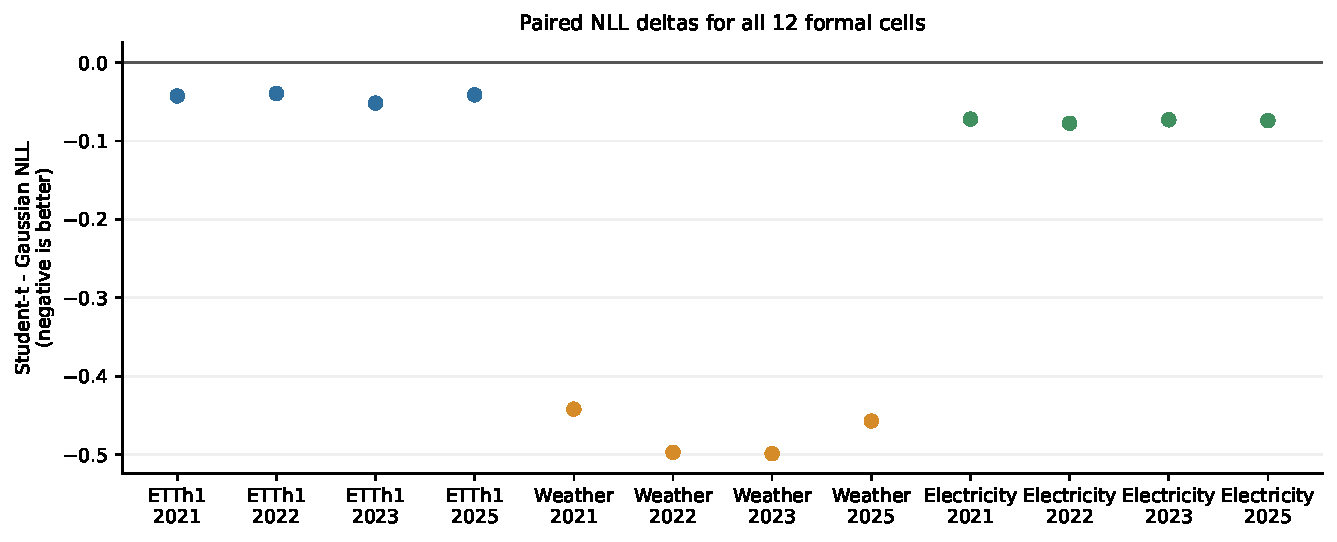
\includegraphics[width=0.96\linewidth]{figures/fig2_multiseed_nll_deltas.pdf}
    \caption{Paired NLL deltas for the TimePerceiver multi-seed matrix. Every displayed delta is negative.}
    \label{fig:multiseed-nll-deltas}
\end{figure}

\begin{figure}[t]
    \centering
    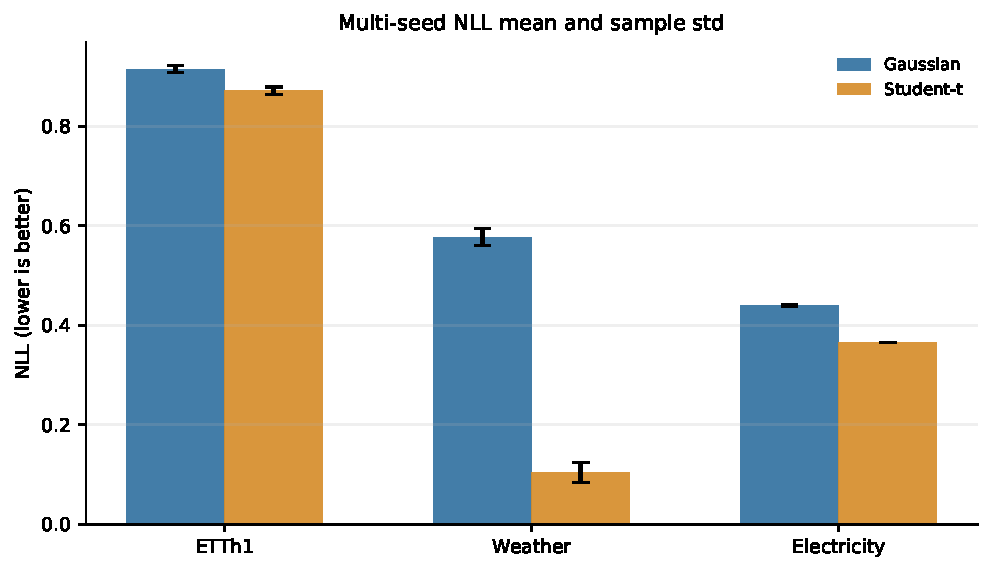
\includegraphics[width=0.32\linewidth]{figures/fig3a_multiseed_nll.pdf}
    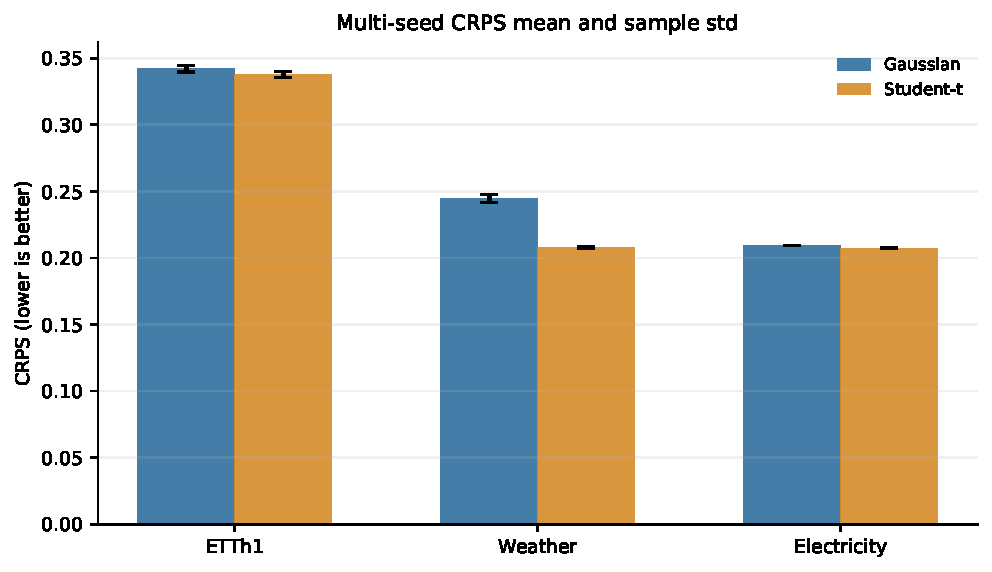
\includegraphics[width=0.32\linewidth]{figures/fig3b_multiseed_crps.pdf}
    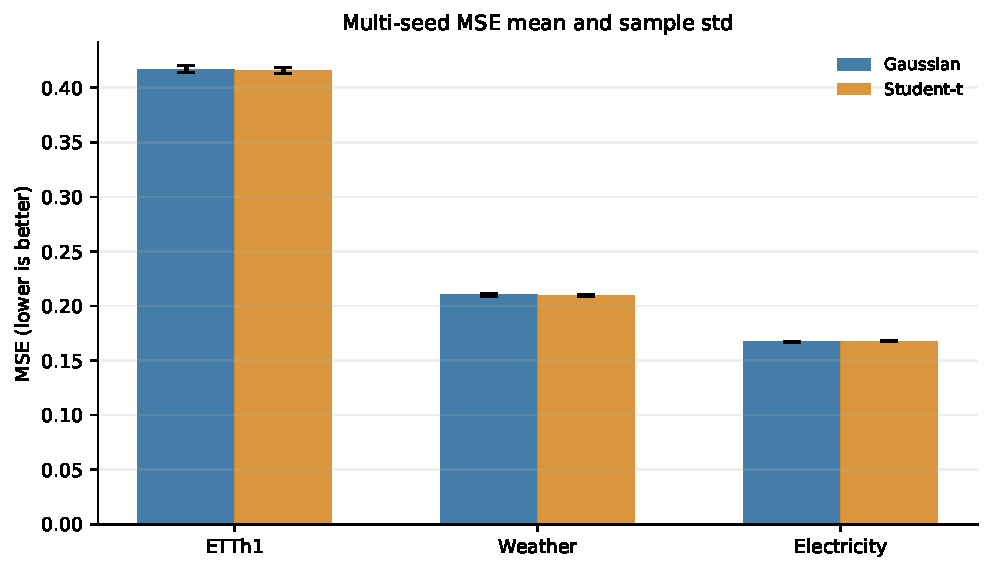
\includegraphics[width=0.32\linewidth]{figures/fig3c_multiseed_mse.pdf}
    \caption{TimePerceiver dataset-level mean and standard-deviation summaries for NLL, CRPS, and MSE across four probability-head training seeds.}
    \label{fig:multiseed-summary}
\end{figure}

\subsection{Distribution-head ablation}
\label{sec:distribution-ablation}

Table~\ref{tab:distribution-ablation} compares Gaussian, Laplace, fixed Student-$t$, and learned-df Student-$t$ heads under random missingness at rate 0.3. The fixed Student-$t$ head records 3/3 NLL wins, 3/3 CRPS-noninferior outcomes, and 3/3 point-noninferior outcomes against Gaussian. The learned-df variant does not consistently improve over fixed df=8. Laplace also lacks equal support across all paired criteria. The formal conclusion is therefore that a fixed heavy-tailed likelihood is sufficient in the evaluated scope.

\begin{table}[t]
    \centering
    \caption{Distribution-head ablation on frozen TimePerceiver checkpoints. The fixed Student-$t$ head uses df=8.}
    \label{tab:distribution-ablation}
    \scriptsize
    \resizebox{\linewidth}{!}{\begin{tabular}{@{}lrrrrrr@{}}
\toprule
Dataset & Head & NLL & CRPS & MSE & Coverage error & Trainable \\
\midrule
etth1 & Gaussian & 0.918535 & 0.344127 & 0.420332 & 0.038132 & 6,168 \\
etth1 & Laplace & 0.879116 & 0.341785 & 0.424149 & 0.011910 & 6,168 \\
etth1 & Fixed Student-t (df=8) & 0.864949 & 0.336548 & 0.413927 & 0.022006 & 6,168 \\
etth1 & Learned Student-t & 0.877154 & 0.340263 & 0.419177 & 0.020301 & 6,175 \\
weather & Gaussian & 0.586325 & 0.245442 & 0.212237 & 0.082667 & 24,624 \\
weather & Laplace & 0.204399 & 0.209589 & 0.210051 & 0.070806 & 24,624 \\
weather & Fixed Student-t (df=8) & 0.136165 & 0.208461 & 0.210994 & 0.051632 & 24,624 \\
weather & Learned Student-t & 0.129293 & 0.208276 & 0.210836 & 0.052156 & 24,645 \\
electricity & Gaussian & 0.440598 & 0.209453 & 0.167881 & 0.038304 & 24,624 \\
electricity & Laplace & 0.370388 & 0.208768 & 0.170436 & 0.018222 & 24,624 \\
electricity & Fixed Student-t (df=8) & 0.367009 & 0.207797 & 0.168473 & 0.018744 & 24,624 \\
electricity & Learned Student-t & 0.366449 & 0.207786 & 0.168486 & 0.018502 & 24,945 \\
\bottomrule
\end{tabular}
}
\end{table}

The fixed Student-$t$ head has the same trainable parameter count as Gaussian and Laplace. Table~\ref{tab:efficiency} reports the controlled parameter, latency, and memory measurements. The learned-df head adds only per-channel shape parameters, yet this extra flexibility does not produce a consistent metric benefit.

\begin{table}[t]
    \centering
    \caption{Controlled probability-head efficiency measurements. Timing comparisons are within each dataset and benchmark environment.}
    \label{tab:efficiency}
    \scriptsize
    \resizebox{\linewidth}{!}{\begin{tabular}{@{}lrrrrrr@{}}
\toprule
Dataset & Head & Params & Forward ms & NLL ms & CRPS ms & Peak MiB \\
\midrule
etth1 & Gaussian & 6,168 & 29.997997 & 51.514500 & 86.934799 & 215.033691 \\
etth1 & Laplace & 6,168 & 29.996887 & 30.016349 & 63.189127 & 215.033691 \\
etth1 & Fixed Student-t (df=8) & 6,168 & 29.902914 & 65.900001 & 90.256716 & 215.034180 \\
etth1 & Learned Student-t & 6,175 & 29.982518 & 69.371223 & 103.335362 & 215.034180 \\
weather & Gaussian & 24,624 & 59.357760 & 79.919755 & 188.685383 & 630.664551 \\
weather & Laplace & 24,624 & 58.485584 & 59.293318 & 133.341993 & 630.664551 \\
weather & Fixed Student-t (df=8) & 24,624 & 58.181018 & 98.037041 & 211.123562 & 630.665039 \\
weather & Learned Student-t & 24,645 & 59.026097 & 97.896011 & 212.516092 & 630.665039 \\
electricity & Gaussian & 24,624 & 356.894562 & 359.007118 & 1248.479182 & 4626.902832 \\
electricity & Laplace & 24,624 & 345.290164 & 343.346301 & 895.849843 & 4626.902832 \\
electricity & Fixed Student-t (df=8) & 24,624 & 343.877731 & 374.742924 & 1477.667372 & 4626.904297 \\
electricity & Learned Student-t & 24,945 & 420.384170 & 473.496327 & 1890.070674 & 4626.904297 \\
\bottomrule
\end{tabular}
}
\end{table}

\subsection{Second-backbone replication}
\label{sec:patchtst-results}

The PatchTST comparison records 3/3 NLL wins, 3/3 CRPS-noninferior outcomes, 2/3 point-noninferior outcomes, and 2/3 full paired passes for the fixed Student-$t$ head. Table~\ref{tab:second-backbone} reports the paired deltas, and Figure~\ref{fig:cross-backbone-deltas} visualizes their signs. ETTh1 and Weather pass every component.

Electricity does not pass the point criterion. Gaussian MSE is 0.165829 and fixed Student-$t$ MSE is 0.167809, a change of +0.001980 or +1.194\%. The increase is above the pre-registered 1\% tolerance in Equation~\ref{eq:point-gate}. The decision is therefore \texttt{SECOND\_BACKBONE\_POINT\_TRADEOFF}. The NLL and CRPS direction transfers to PatchTST, but the complete multi-metric gate does not.

\begin{table}[t]
    \centering
    \caption{Within-backbone deltas for fixed Student-$t$ versus Gaussian. The point threshold permits at most a 1\% relative MSE increase.}
    \label{tab:second-backbone}
    \scriptsize
    \resizebox{\linewidth}{!}{\begin{tabular}{@{}lrrrrrrrrr@{}}
\toprule
Dataset & Backbone & $\Delta$NLL & $\Delta$CRPS & $\Delta$MSE & Rel. MSE & NLL win & CRPS NI & Point NI & Full pair \\
\midrule
ETTh1 & TimePerceiver & -0.053587 & -0.007578 & -0.006405 & -1.524\% & Yes & Yes & Yes & Yes \\
ETTh1 & PatchTST & -0.035317 & -0.002538 & -0.005439 & -1.274\% & Yes & Yes & Yes & Yes \\
Weather & TimePerceiver & -0.450160 & -0.036981 & -0.001243 & -0.586\% & Yes & Yes & Yes & Yes \\
Weather & PatchTST & -1.818698 & -0.076205 & -0.050179 & -21.595\% & Yes & Yes & Yes & Yes \\
Electricity & TimePerceiver & -0.073589 & -0.001656 & 0.000592 & +0.353\% & Yes & Yes & Yes & Yes \\
Electricity & PatchTST & -0.083433 & -0.001688 & 0.001980 & +1.194\% & Yes & Yes & No & No \\
\bottomrule
\end{tabular}
}
\end{table}

\begin{figure}[t]
    \centering
    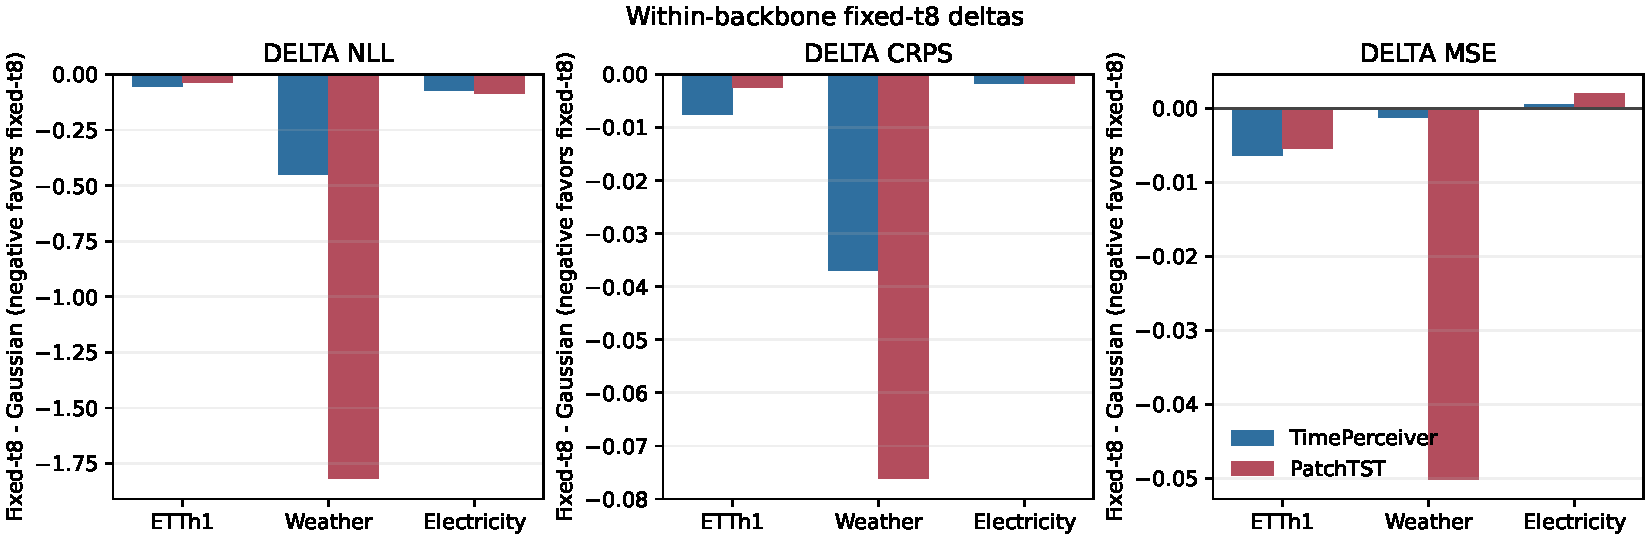
\includegraphics[width=0.96\linewidth]{figures/fig_gate5b_cross_backbone_deltas.pdf}
    \caption{Within-backbone metric deltas. Negative values favor the fixed Student-$t$ head. PatchTST NLL and CRPS improve on all three datasets, while Electricity has a small positive MSE delta.}
    \label{fig:cross-backbone-deltas}
\end{figure}

\subsection{Heavy-tail diagnostics}
\label{sec:tail-diagnostics}

Residual-percentile diagnostics indicate that much of the NLL gain appears in the most extreme Gaussian-residual region. Figure~\ref{fig:tail-nll} shows this pattern for the TimePerceiver ablation. The corresponding PatchTST diagnostic covers approximately $1.82\times10^8$ forecast elements and yields the same qualitative concentration in its most extreme bin. These analyses are descriptive. They are not formal gate evidence, causal mechanism tests, or inferential samples of $1.82\times10^8$ independent observations.

\begin{figure}[t]
    \centering
    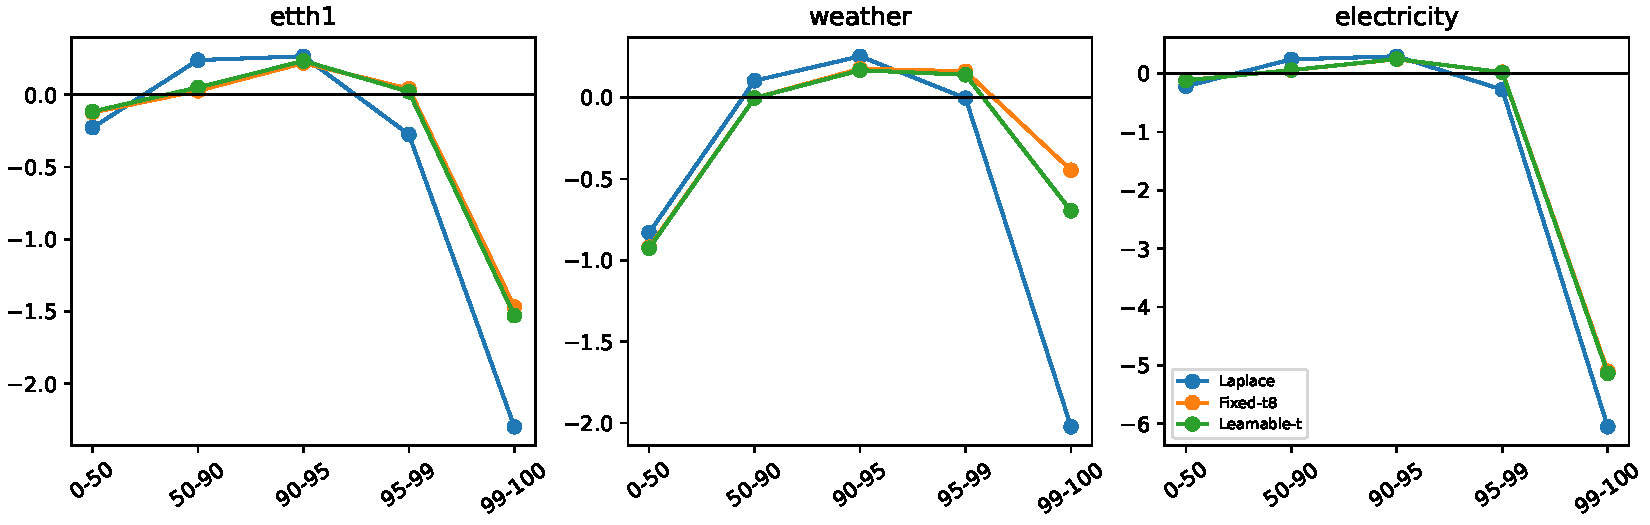
\includegraphics[width=0.90\linewidth]{figures/fig_gate5a_tail_nll_gain.pdf}
    \caption{Descriptive NLL differences across Gaussian-residual percentile bins for the TimePerceiver distribution ablation.}
    \label{fig:tail-nll}
\end{figure}

\section{Ablations and Negative Results}
\label{sec:negative-results}

\subsection{Missingness-aware FiLM}

The frozen-backbone static adapter improves ETTh1 random-0.3 MSE from 0.425394 to 0.361377. A missingness-aware FiLM adapter reaches 0.363156, which is 0.001778 worse than the static adapter. The mechanism audit finds a nonconstant condition representation, nonzero FiLM modulation, finite gradients, and updated conditioning parameters. These checks do not support an optimization or gradient-flow failure.

The supported interpretation is narrower: the tested global-statistics FiLM conditioning adds no generalization value beyond matched static capacity in this fixed condition. It does not rule out local temporal or channel-structured conditioning. Detailed adapter results are retained in Appendix~\ref{app:adapter}.

\subsection{Additive split conformal calibration}

The conformal experiment uses a strict raw-time selection and calibration split with a 479-row embargo. Native test intervals are already near their nominal targets, while the calibration segment is descriptively harder. The evaluated additive correction has a nonnegative quantile and can only expand intervals. In this setting, expansion moves native test intervals toward overcoverage, increases width, and worsens both absolute coverage error and interval score.

Figure~\ref{fig:conformal-tradeoff} displays the tradeoff. Mask-severity conditioning changes bin-specific quantiles but does not repair the aggregate result. A test-label shrinkage calculation is retained only as a counterfactual diagnosis and is not a valid calibrator. This finding is specific to the additive score, split, dataset, and missingness condition.

\begin{figure}[t]
    \centering
    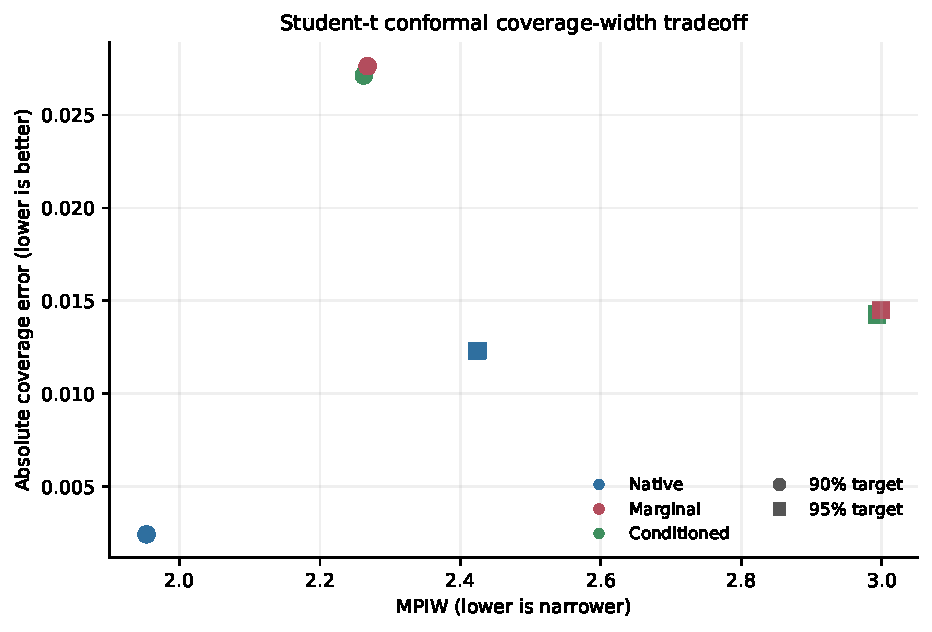
\includegraphics[width=0.88\linewidth]{figures/fig5_conformal_tradeoff.pdf}
    \caption{Native and additive conformal interval tradeoffs under the strict ETTh1 random-0.3 split. The additive procedures widen intervals without improving absolute coverage error.}
    \label{fig:conformal-tradeoff}
\end{figure}

\subsection{PatchTST point-prediction tradeoff}

The PatchTST Electricity result is not removed because its probabilistic scores improve. It is instead reported as a partial transfer result: NLL and CRPS improve, while relative MSE increases by 1.194\%. This single threshold miss changes the complete second-backbone decision from positive to a point-prediction tradeoff.

\section{Limitations}
\label{sec:limitations}

\begin{enumerate}
    \item The study covers three datasets: ETTh1, Weather, and Electricity.
    \item It evaluates two backbones, TimePerceiver and PatchTST.
    \item Fixed test masks support pairing but do not represent every possible missingness realization.
    \item Several expanded conditions use one probability-head training seed.
    \item The TimePerceiver multi-seed matrix keeps each official backbone checkpoint fixed.
    \item PatchTST uses one clean-backbone seed and one probability-head seed.
    \item The PatchTST study is limited to random missingness at rate 0.3.
    \item No inferential significance analysis is reported.
    \item The probability heads model marginal target-element distributions.
    \item Cross-channel and cross-horizon covariance are not modeled.
    \item Marginal interval coverage does not establish simultaneous channel or horizon coverage.
    \item Fixed df=8 is empirically sufficient here but is not a theoretical optimum.
    \item The complete second-backbone gate fails because Electricity MSE increases by 1.194\%.
    \item The conformal result concerns one additive split procedure on ETTh1 random-0.3.
    \item The FiLM result concerns one global-statistics conditioning design and one insertion pattern.
\end{enumerate}

These boundaries define the evidence rather than post-hoc exceptions. Broader backbone seeds, missingness realizations, distribution shifts, and covariance-aware heads remain open evaluation directions.

\section{Conclusion}
\label{sec:conclusion}

The evidence supports fixed heavy-tailed probabilistic forecasting under missing historical observations. The fixed missing-history protocol controls masks, normalization, model selection, and target access. On TimePerceiver, Student-$t$ variants improve NLL and CRPS across three datasets and four probability-head training seeds. The distribution ablation supports fixed df=8 as sufficient under the evaluated setting.

On PatchTST, the fixed Student-$t$ head improves NLL and CRPS on all three datasets. However, the Electricity point-prediction tradeoff prevents the complete second-backbone gate from being positive. The final evidence therefore supports probabilistic-score robustness across the two evaluated backbones, but it does not establish metric-wise invariance beyond them.


\bibliographystyle{plain}
\bibliography{references}

\appendix
\section{Additional Evidence and Reproducibility}
\label{app:appendix}

\subsection{Additional Results}
\label{app:additional-results}

\subsubsection{Adapter ablation}
\label{app:adapter}

Table~\ref{tab:adapter-ablation} gives the full Gate 4a comparison. Figure~\ref{fig:adapter-ablation} visualizes the same test MSE values. The missingness-aware FiLM branch is active, but it does not outperform the static adapter.

\begin{table}[ht]
    \centering
    \caption{Gate 4a adapter comparison on ETTh1 random-0.3.}
    \label{tab:adapter-ablation}
    \scriptsize
    \begin{tabular}{@{}lrrrrrr@{}}
\toprule
Variant & Trainable & Overhead & Best epoch & Val. MSE & Test MSE & Test MAE \\
\midrule
Official & 0 & 0.00\% & NA & NA & 0.425394 & 0.450336 \\
Static adapter & 33,600 & 2.96\% & 1 & 0.678666 & 0.361377 & 0.390458 \\
Missingness-aware FiLM adapter & 39,136 & 3.44\% & 5 & 0.679754 & 0.363156 & 0.391077 \\
\bottomrule
\end{tabular}

\end{table}

\begin{figure}[ht]
    \centering
    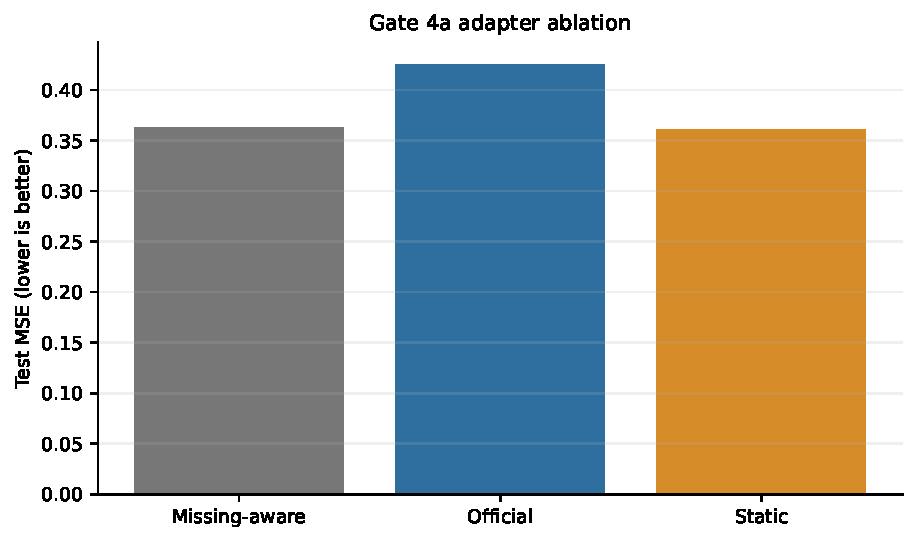
\includegraphics[width=0.78\linewidth]{figures/figA1_gate4a_adapter.pdf}
    \caption{Static and missingness-aware adapter results relative to the official reference.}
    \label{fig:adapter-ablation}
\end{figure}

\subsubsection{Cross-condition TimePerceiver evidence}

Table~\ref{tab:etth1-cross-condition} reports the ETTh1 condition matrix. It uses the same fixed evaluation assets for Gaussian and Student-$t$ heads within each condition.

\begin{table}[ht]
    \centering
    \caption{ETTh1 cross-condition paired comparison.}
    \label{tab:etth1-cross-condition}
    \scriptsize
    \resizebox{\linewidth}{!}{\begin{tabular}{@{}lrrrrrr@{}}
\toprule
Condition & $\Delta$NLL & $\Delta$CRPS & $\Delta$MSE & NLL win & CRPS NI & Point NI \\
\midrule
Random 0.1 & -0.078025 & -0.006113 & -0.002231 & Yes & Yes & Yes \\
Random 0.3 & -0.041381 & -0.003864 & -0.001155 & Yes & Yes & Yes \\
Random 0.5 & -0.013720 & 0.000656 & 0.007100 & Yes & No & No \\
Block 0.3 & -0.061086 & -0.007738 & -0.004834 & Yes & Yes & Yes \\
Channel 0.3 & -0.071504 & -0.004849 & 0.001022 & Yes & Yes & Yes \\
Mixed 0.3 & -0.070665 & -0.003286 & 0.001169 & Yes & Yes & Yes \\
\bottomrule
\end{tabular}
}
\end{table}

\subsubsection{Conformal details}

Tables~\ref{tab:conformal-main} and~\ref{tab:conformal-mechanism} retain the formal conformal results and mechanism audit. Figure~\ref{fig:calibration-shift} compares calibration and test coverage. Figures~\ref{fig:channel-coverage} and~\ref{fig:horizon-coverage} show channel- and horizon-level diagnostics.

\begin{table}[ht]
    \centering
    \caption{Formal additive conformal results.}
    \label{tab:conformal-main}
    \scriptsize
    \begin{tabular}{@{}lrrrrr@{}}
\toprule
Method & Nominal & PICP & MPIW & Coverage error & Interval score \\
\midrule
Mask-severity-conditioned conformal & 0.90 & 0.927136 & 2.262613 & 0.027136 & 2.989775 \\
Marginal conformal & 0.90 & 0.927636 & 2.267989 & 0.027636 & 2.990528 \\
Native & 0.90 & 0.897581 & 1.953189 & 0.002419 & 2.946898 \\
Mask-severity-conditioned conformal & 0.95 & 0.964262 & 2.993500 & 0.014262 & 3.625242 \\
Marginal conformal & 0.95 & 0.964505 & 2.998730 & 0.014505 & 3.625259 \\
Native & 0.95 & 0.937700 & 2.424187 & 0.012300 & 3.596873 \\
\bottomrule
\end{tabular}

\end{table}

\begin{table}[ht]
    \centering
    \caption{Conformal mechanism audit. Counterfactual values are diagnostic and not formal calibration.}
    \label{tab:conformal-mechanism}
    \scriptsize
    \resizebox{\linewidth}{!}{\begin{tabular}{@{}lrrrrrr@{}}
\toprule
Head & Nominal & Cal. PICP & Test PICP & Shift & $\hat q$ & $\Delta$ coverage error \\
\midrule
Gaussian & 0.90 & 0.869114 & 0.904533 & 0.035418 & 0.126842 & 0.023728 \\
Gaussian & 0.95 & 0.912017 & 0.937263 & 0.025246 & 0.279881 & 0.001974 \\
Student-t & 0.90 & 0.861667 & 0.897581 & 0.035913 & 0.157400 & 0.025216 \\
Student-t & 0.95 & 0.913178 & 0.937700 & 0.024522 & 0.287271 & 0.002205 \\
\bottomrule
\end{tabular}
}
\end{table}

\begin{figure}[ht]
    \centering
    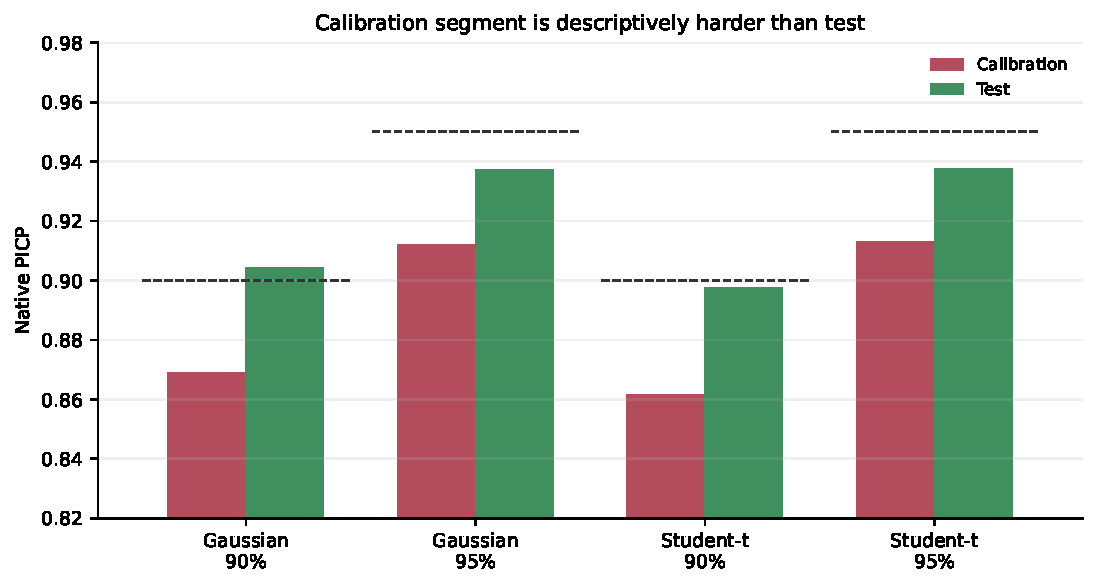
\includegraphics[width=0.78\linewidth]{figures/fig6_calibration_test_shift.pdf}
    \caption{Descriptive calibration-to-test coverage shift under the strict temporal split.}
    \label{fig:calibration-shift}
\end{figure}

\begin{figure}[ht]
    \centering
    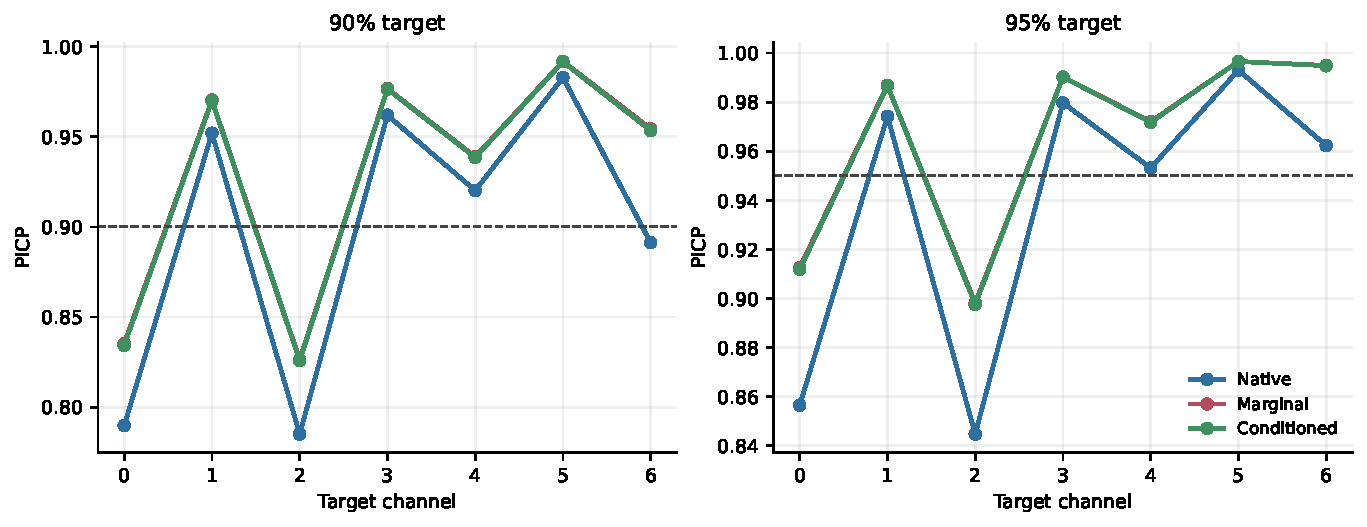
\includegraphics[width=0.48\linewidth]{figures/figA2_gate4c_channel_coverage.pdf}
    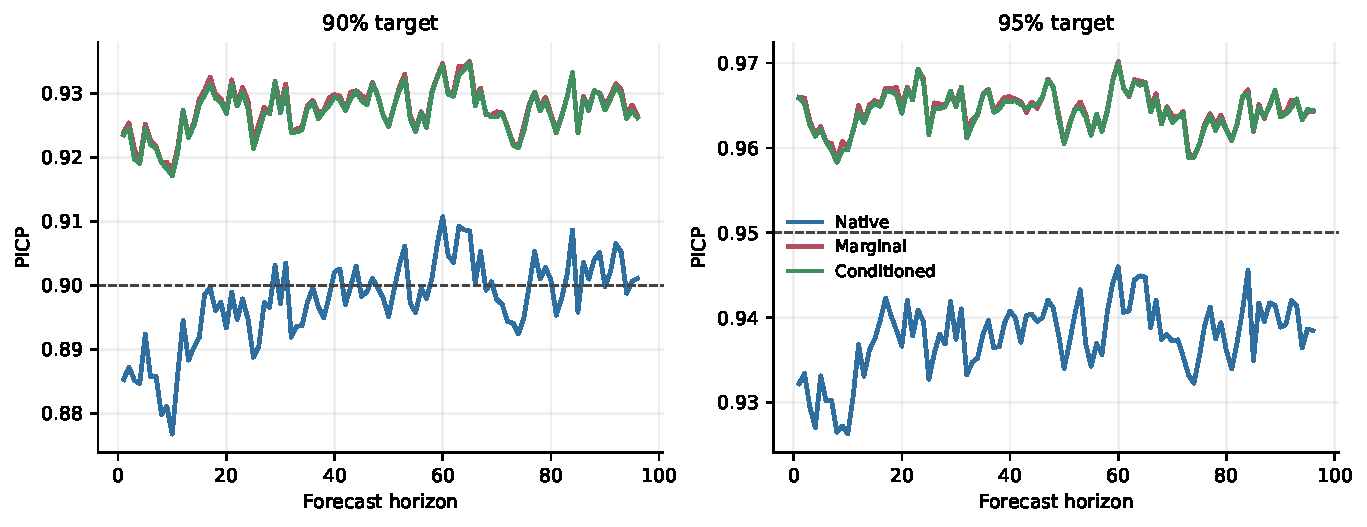
\includegraphics[width=0.48\linewidth]{figures/figA3_gate4c_horizon_coverage.pdf}
    \caption{Channel-level and horizon-level coverage diagnostics for the Gate 4c experiment.}
    \label{fig:channel-coverage}
    \label{fig:horizon-coverage}
\end{figure}

\subsubsection{Complete fixed-mask degradation matrix}

Tables~\ref{tab:full-mask-etth1}--\ref{tab:full-mask-electricity} retain every Gate 3b cell while splitting the matrix by dataset for readability.

\begin{table}[ht]
    \centering
    \caption{Full ETTh1 fixed-mask degradation matrix.}
    \label{tab:full-mask-etth1}
    \scriptsize
    \begin{tabular}{@{}lrrrr@{}}
\toprule
Mask & Rate & MSE & MAE & RMSE \\
\midrule
Block & 0.10 & 0.388818 & 0.416915 & 0.623552 \\
Block & 0.30 & 0.423837 & 0.451188 & 0.651027 \\
Block & 0.50 & 0.486504 & 0.501242 & 0.697498 \\
Block & 0.70 & 0.591697 & 0.571655 & 0.769219 \\
Channel & 0.10 & 0.479410 & 0.455063 & 0.692394 \\
Channel & 0.30 & 0.583704 & 0.511084 & 0.764006 \\
Channel & 0.50 & 0.798862 & 0.627325 & 0.893791 \\
Channel & 0.70 & 0.900947 & 0.683061 & 0.949182 \\
Mixed & 0.10 & 0.486209 & 0.464128 & 0.697287 \\
Mixed & 0.30 & 0.495055 & 0.473908 & 0.703601 \\
Mixed & 0.50 & 0.553485 & 0.525226 & 0.743966 \\
Mixed & 0.70 & 0.715806 & 0.617339 & 0.846053 \\
Random & 0.10 & 0.378811 & 0.408069 & 0.615476 \\
Random & 0.30 & 0.425394 & 0.450336 & 0.652223 \\
Random & 0.50 & 0.525856 & 0.523115 & 0.725160 \\
Random & 0.70 & 0.688520 & 0.617690 & 0.829771 \\
\bottomrule
\end{tabular}

\end{table}

\begin{table}[ht]
    \centering
    \caption{Full Weather fixed-mask degradation matrix.}
    \label{tab:full-mask-weather}
    \scriptsize
    \begin{tabular}{@{}lrrrr@{}}
\toprule
Mask & Rate & MSE & MAE & RMSE \\
\midrule
Block & 0.10 & 0.158302 & 0.218956 & 0.397872 \\
Block & 0.30 & 0.180420 & 0.245178 & 0.424759 \\
Block & 0.50 & 0.210474 & 0.277453 & 0.458774 \\
Block & 0.70 & 0.254572 & 0.322297 & 0.504551 \\
Channel & 0.10 & 0.191289 & 0.238851 & 0.437366 \\
Channel & 0.30 & 0.284471 & 0.316355 & 0.533358 \\
Channel & 0.50 & 0.377902 & 0.393866 & 0.614738 \\
Channel & 0.70 & 0.495709 & 0.490618 & 0.704066 \\
Mixed & 0.10 & 0.175815 & 0.230739 & 0.419303 \\
Mixed & 0.30 & 0.224939 & 0.281431 & 0.474278 \\
Mixed & 0.50 & 0.306930 & 0.357264 & 0.554012 \\
Mixed & 0.70 & 0.400193 & 0.440502 & 0.632608 \\
Random & 0.10 & 0.169631 & 0.232543 & 0.411863 \\
Random & 0.30 & 0.240810 & 0.309629 & 0.490724 \\
Random & 0.50 & 0.331313 & 0.391138 & 0.575598 \\
Random & 0.70 & 0.434543 & 0.474367 & 0.659199 \\
\bottomrule
\end{tabular}

\end{table}

\begin{table}[ht]
    \centering
    \caption{Full Electricity fixed-mask degradation matrix.}
    \label{tab:full-mask-electricity}
    \scriptsize
    \begin{tabular}{@{}lrrrr@{}}
\toprule
Mask & Rate & MSE & MAE & RMSE \\
\midrule
Block & 0.10 & 0.143247 & 0.243795 & 0.378480 \\
Block & 0.30 & 0.184630 & 0.289155 & 0.429686 \\
Block & 0.50 & 0.270835 & 0.369677 & 0.520418 \\
Block & 0.70 & 0.464169 & 0.520260 & 0.681300 \\
Channel & 0.10 & 0.213972 & 0.281108 & 0.462571 \\
Channel & 0.30 & 0.391038 & 0.403166 & 0.625331 \\
Channel & 0.50 & 0.569116 & 0.525639 & 0.754398 \\
Channel & 0.70 & 0.748916 & 0.649662 & 0.865399 \\
Mixed & 0.10 & 0.165759 & 0.254616 & 0.407135 \\
Mixed & 0.30 & 0.246785 & 0.325159 & 0.496775 \\
Mixed & 0.50 & 0.375182 & 0.437690 & 0.612521 \\
Mixed & 0.70 & 0.588662 & 0.596810 & 0.767243 \\
Random & 0.10 & 0.138429 & 0.242728 & 0.372060 \\
Random & 0.30 & 0.200572 & 0.318891 & 0.447853 \\
Random & 0.50 & 0.325732 & 0.432183 & 0.570729 \\
Random & 0.70 & 0.546080 & 0.584678 & 0.738972 \\
\bottomrule
\end{tabular}

\end{table}

\subsubsection{All conformal heads}

Table~\ref{tab:all-conformal-heads} reports every retained head and interval method. Extra probability diagnostics are shown in Figures~\ref{fig:pit-diagnostic}--\ref{fig:patchtst-tail}.

\begin{table}[ht]
    \centering
    \caption{All Gate 4c head and interval-method combinations.}
    \label{tab:all-conformal-heads}
    \scriptsize
    \resizebox{\linewidth}{!}{\begin{tabular}{@{}lrrrrrr@{}}
\toprule
Head & Method & Nominal & PICP & MPIW & Coverage error & Interval score \\
\midrule
Gaussian & Mask-severity-conditioned conformal & 0.90 & 0.927797 & 2.289391 & 0.027797 & 2.979145 \\
Gaussian & Marginal conformal & 0.90 & 0.928261 & 2.294196 & 0.028261 & 2.979930 \\
Gaussian & Native & 0.90 & 0.904533 & 2.040512 & 0.004533 & 2.936425 \\
Gaussian & Mask-severity-conditioned conformal & 0.95 & 0.964530 & 2.986506 & 0.014530 & 3.598434 \\
Gaussian & Marginal conformal & 0.95 & 0.964711 & 2.991181 & 0.014711 & 3.598406 \\
Gaussian & Native & 0.95 & 0.937263 & 2.431420 & 0.012737 & 3.571486 \\
Student-t & Mask-severity-conditioned conformal & 0.90 & 0.927136 & 2.262613 & 0.027136 & 2.989775 \\
Student-t & Marginal conformal & 0.90 & 0.927636 & 2.267989 & 0.027636 & 2.990528 \\
Student-t & Native & 0.90 & 0.897581 & 1.953189 & 0.002419 & 2.946898 \\
Student-t & Mask-severity-conditioned conformal & 0.95 & 0.964262 & 2.993500 & 0.014262 & 3.625242 \\
Student-t & Marginal conformal & 0.95 & 0.964505 & 2.998730 & 0.014505 & 3.625259 \\
Student-t & Native & 0.95 & 0.937700 & 2.424187 & 0.012300 & 3.596873 \\
\bottomrule
\end{tabular}
}
\end{table}

\begin{figure}[ht]
    \centering
    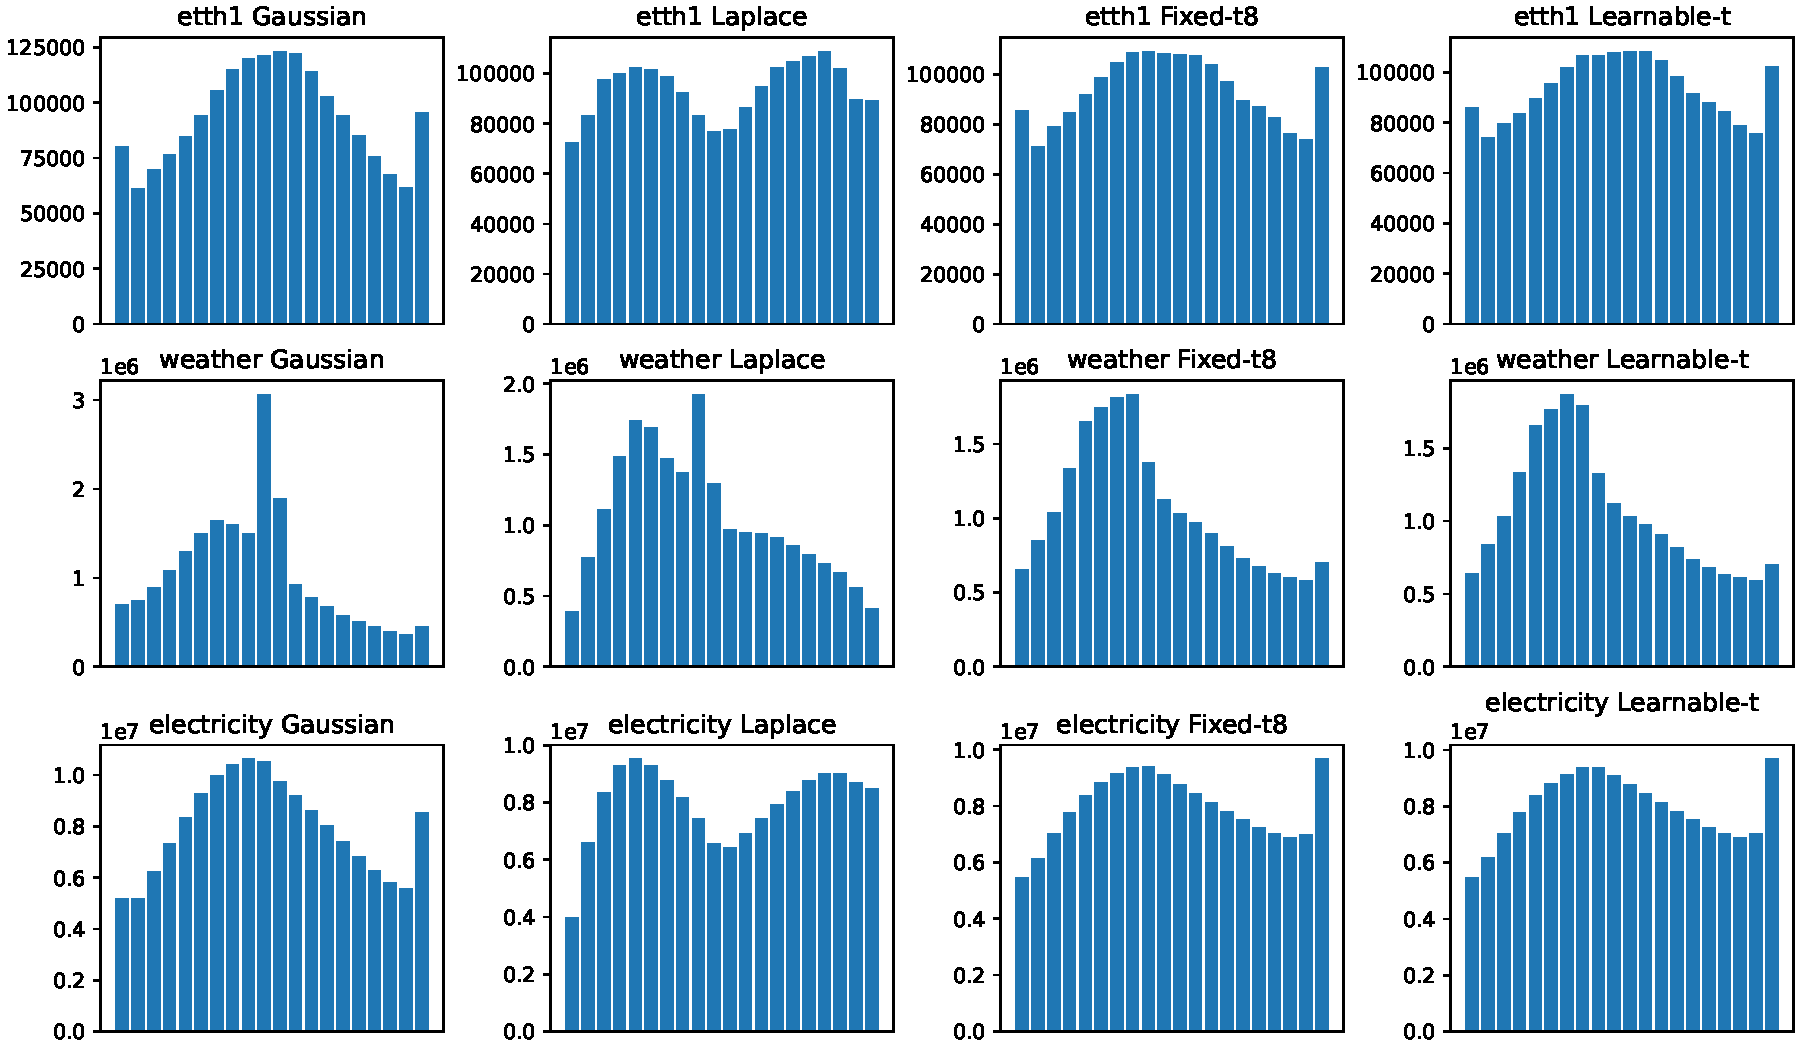
\includegraphics[width=0.48\linewidth]{figures/fig_gate5a_pit_histograms.pdf}
    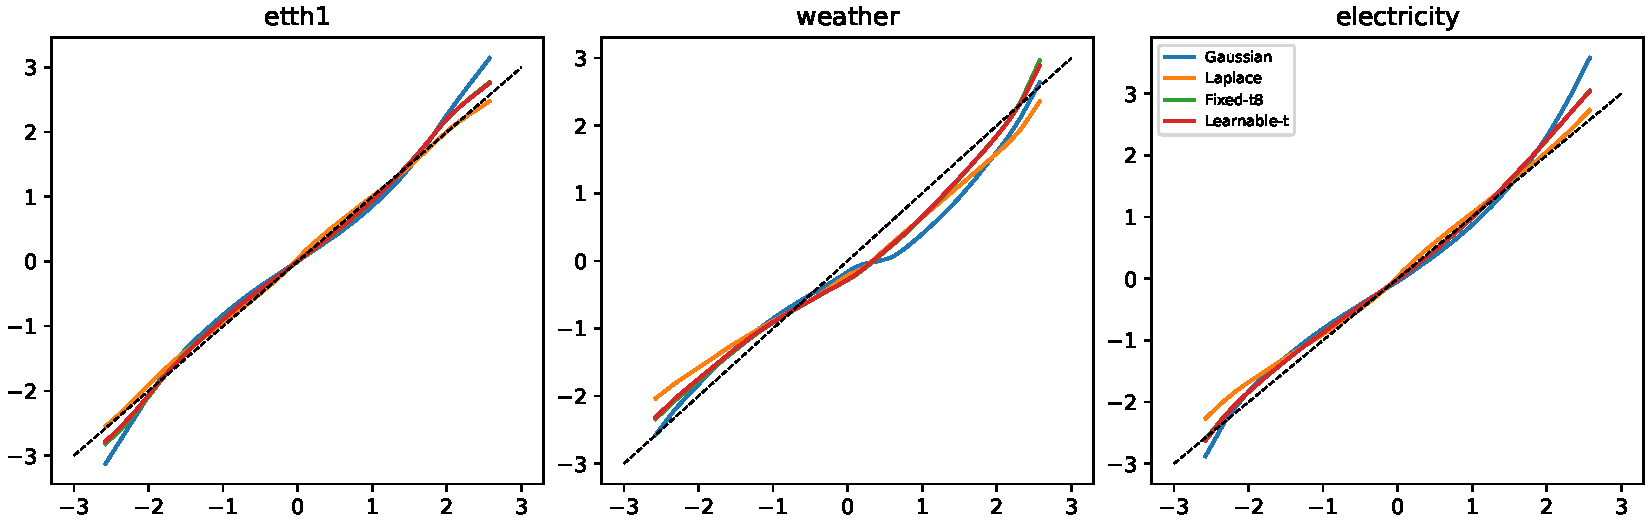
\includegraphics[width=0.48\linewidth]{figures/fig_gate5a_qq.pdf}
    \caption{Descriptive probability integral transform and quantile diagnostics.}
    \label{fig:pit-diagnostic}
\end{figure}

\begin{figure}[ht]
    \centering
    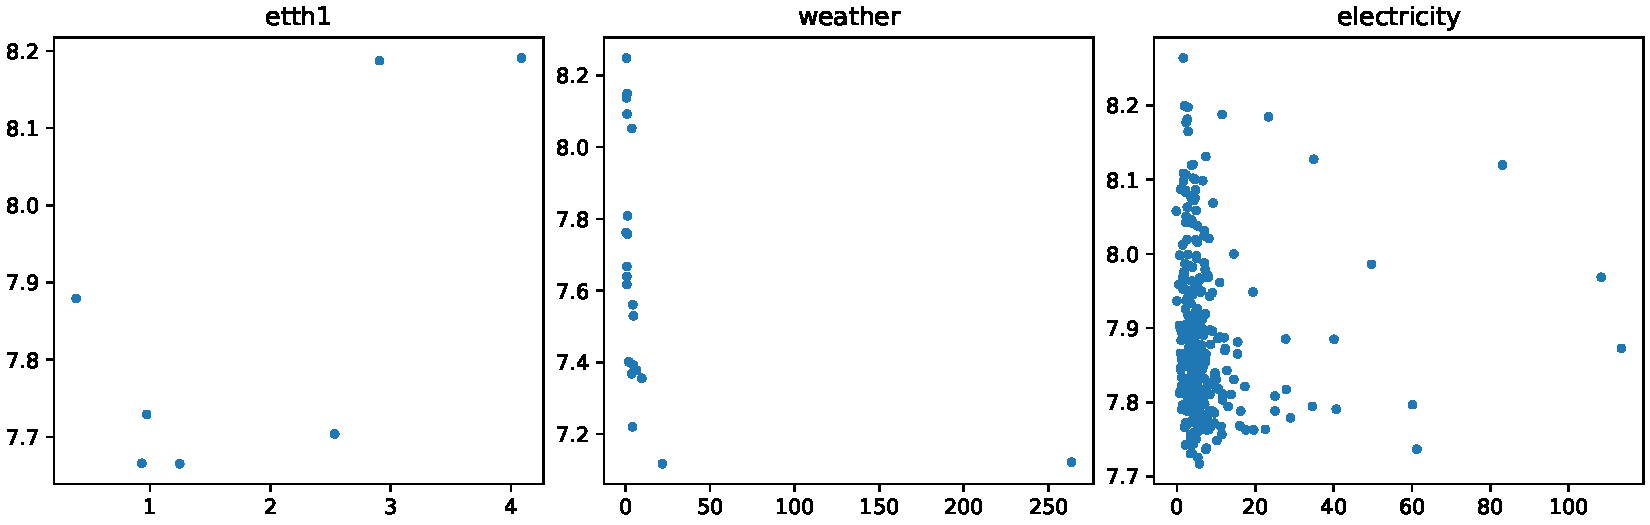
\includegraphics[width=0.48\linewidth]{figures/fig_gate5a_kurtosis_df.pdf}
    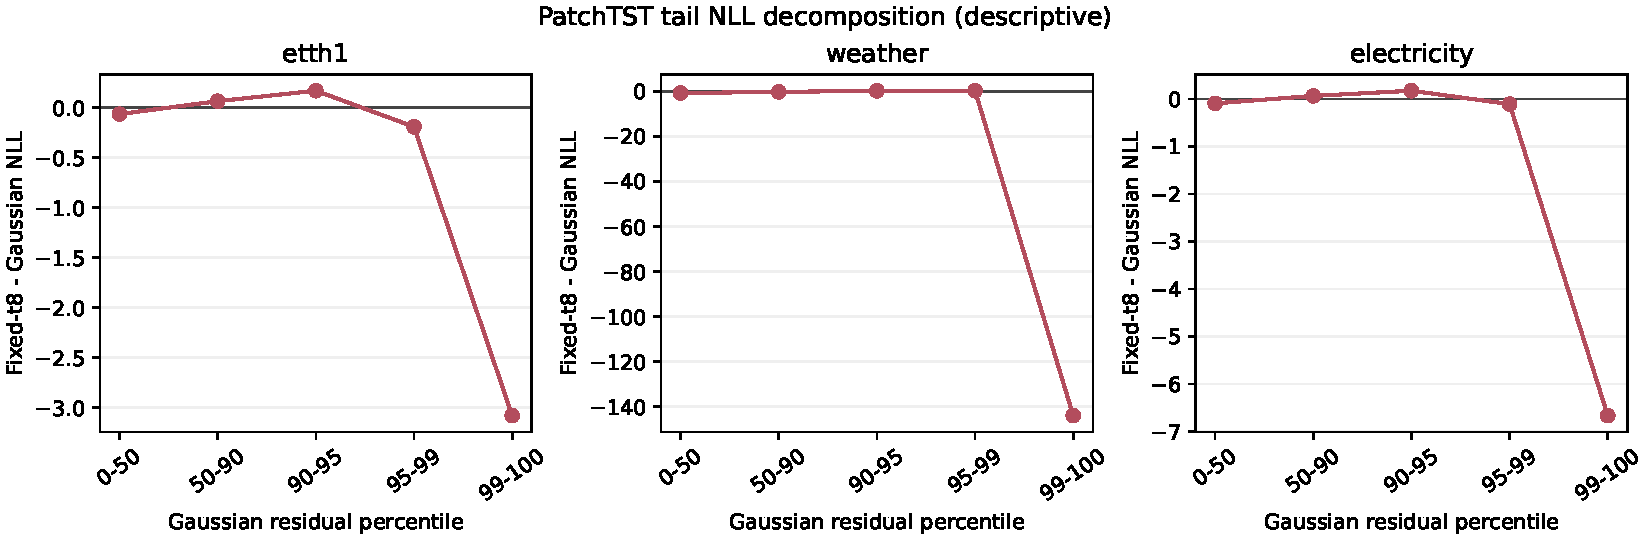
\includegraphics[width=0.48\linewidth]{figures/fig_gate5b_patchtst_tail_nll_gain.pdf}
    \caption{Channel-tail diagnostics and the descriptive PatchTST residual-percentile NLL decomposition.}
    \label{fig:patchtst-tail}
\end{figure}

\subsection{Protocol Details}
\label{app:protocol}

The input length is 384 and the prediction length is 96 throughout the formal study. Dataset boundaries follow the official backbone implementations. Training-only normalization is frozen before validation or test access. Historical masks are applied after constructing the input window and before the backbone forward pass. Target windows are copied before masking and verified unchanged.

Random masks remove individual historical elements. Block masks remove contiguous temporal regions. Channel masks remove complete historical channels. Mixed masks combine mechanisms under the recorded rate. The test-mask seed is 2025. Matched methods load the same mask files and hashes.

Probability heads are selected by validation NLL. CRPS uses 64 MC samples and seed 52025. Native intervals use each distribution's marginal quantiles. The Gate 4c calibration segment follows the selection segment and is separated by a 479-row embargo. Test labels are excluded from calibration.

The paired point criterion allows at most a 1\% relative MSE increase. This criterion is applied identically to TimePerceiver and PatchTST. It is the reason PatchTST Electricity remains a failed point-noninferiority cell despite improved NLL and CRPS.

\subsection{Reproducibility Record}
\label{app:reproducibility}

The anonymous evidence package records the resolved configuration, random seed, checkpoint hash, validation-mask hash, test-mask hash, training-protocol hash, metric-protocol hash, and source row for every formal paper result. Invalid historical runs that did not apply the input mask remain in the internal audit registry and are excluded from all manuscript tables, figures, claims, and reproduction assets.

The TimePerceiver source commit is \texttt{7e30cc07b51c709f408409fd60a34c81ae8990be}. The PatchTST source commit is \texttt{204c21efe0b39603ad6e2ca640ef5896646ab1a9}. The recorded software environment uses Python 3.9.25, PyTorch 2.1.0 with CUDA runtime 12.1, and fixed metric implementations. Public code locations will replace the anonymous placeholder after review.



\end{document}
